\documentclass[12pt,a4paper]{beamer}
\usetheme{Berlin}
\usepackage{amsmath}
\usepackage{amsfonts}
\usepackage{amssymb}
\usepackage[utf8]{inputenc}
\usepackage[polish]{babel}
\usepackage[T1]{fontenc}
\usepackage{graphicx}
\author{Mateusz Katuszonek}
\title{Projekt sytemu informatycznego}
\logo{
\includegraphics[scale=0.2]{zut.jpg}}
\institute{Wydzial Informatyki ZUT}
\date{\today}

\begin{document}
\begin{frame}
\maketitle
Promotor dr Jan Niezbedny\\
Recenzent dr Jan Jakiśtam
\end{frame}
\begin{frame}{Plan prezentacji}
    \tableofcontents
\end{frame}
\section{Wstęp}
\begin{frame}{Wstęp}
    \begin{block}{Cel Pracy}
    asdasdas
    \end{block}
   \begin{alertblock}{Zakres Pracy}
    123456789
    \end{alertblock}
\end{frame}
\section{Projekt Systemu Informatycznego}
\begin{frame}{Projekt Systemu Informatycznego}
    \begin{itemize}
        \item punkt 1
        \item punkt 2
    \end{itemize}
    \begin{table}[h]
    \centering
    \caption{Jakaś tabelka}
    \begin{tabular}{|r|c|c|c|c|}
    \hline
        Jakieś wartości &1&2&3&4\\
        \hline
        Inne wartości &5&6&7&8\\ 
        \hline
        Jeszcze inne &9&10&11&12\\
        \hline
    \end{tabular}
    \end{table}
\end{frame}
\begin{frame}{Projekt Systemu Informatycznego}
    \begin{block}
        
    \end{block}
\end{frame}
\section{Wyniki testowania}
\begin{frame}{Wyniki testowania}
    \begin{figure}[h]
    \centering
    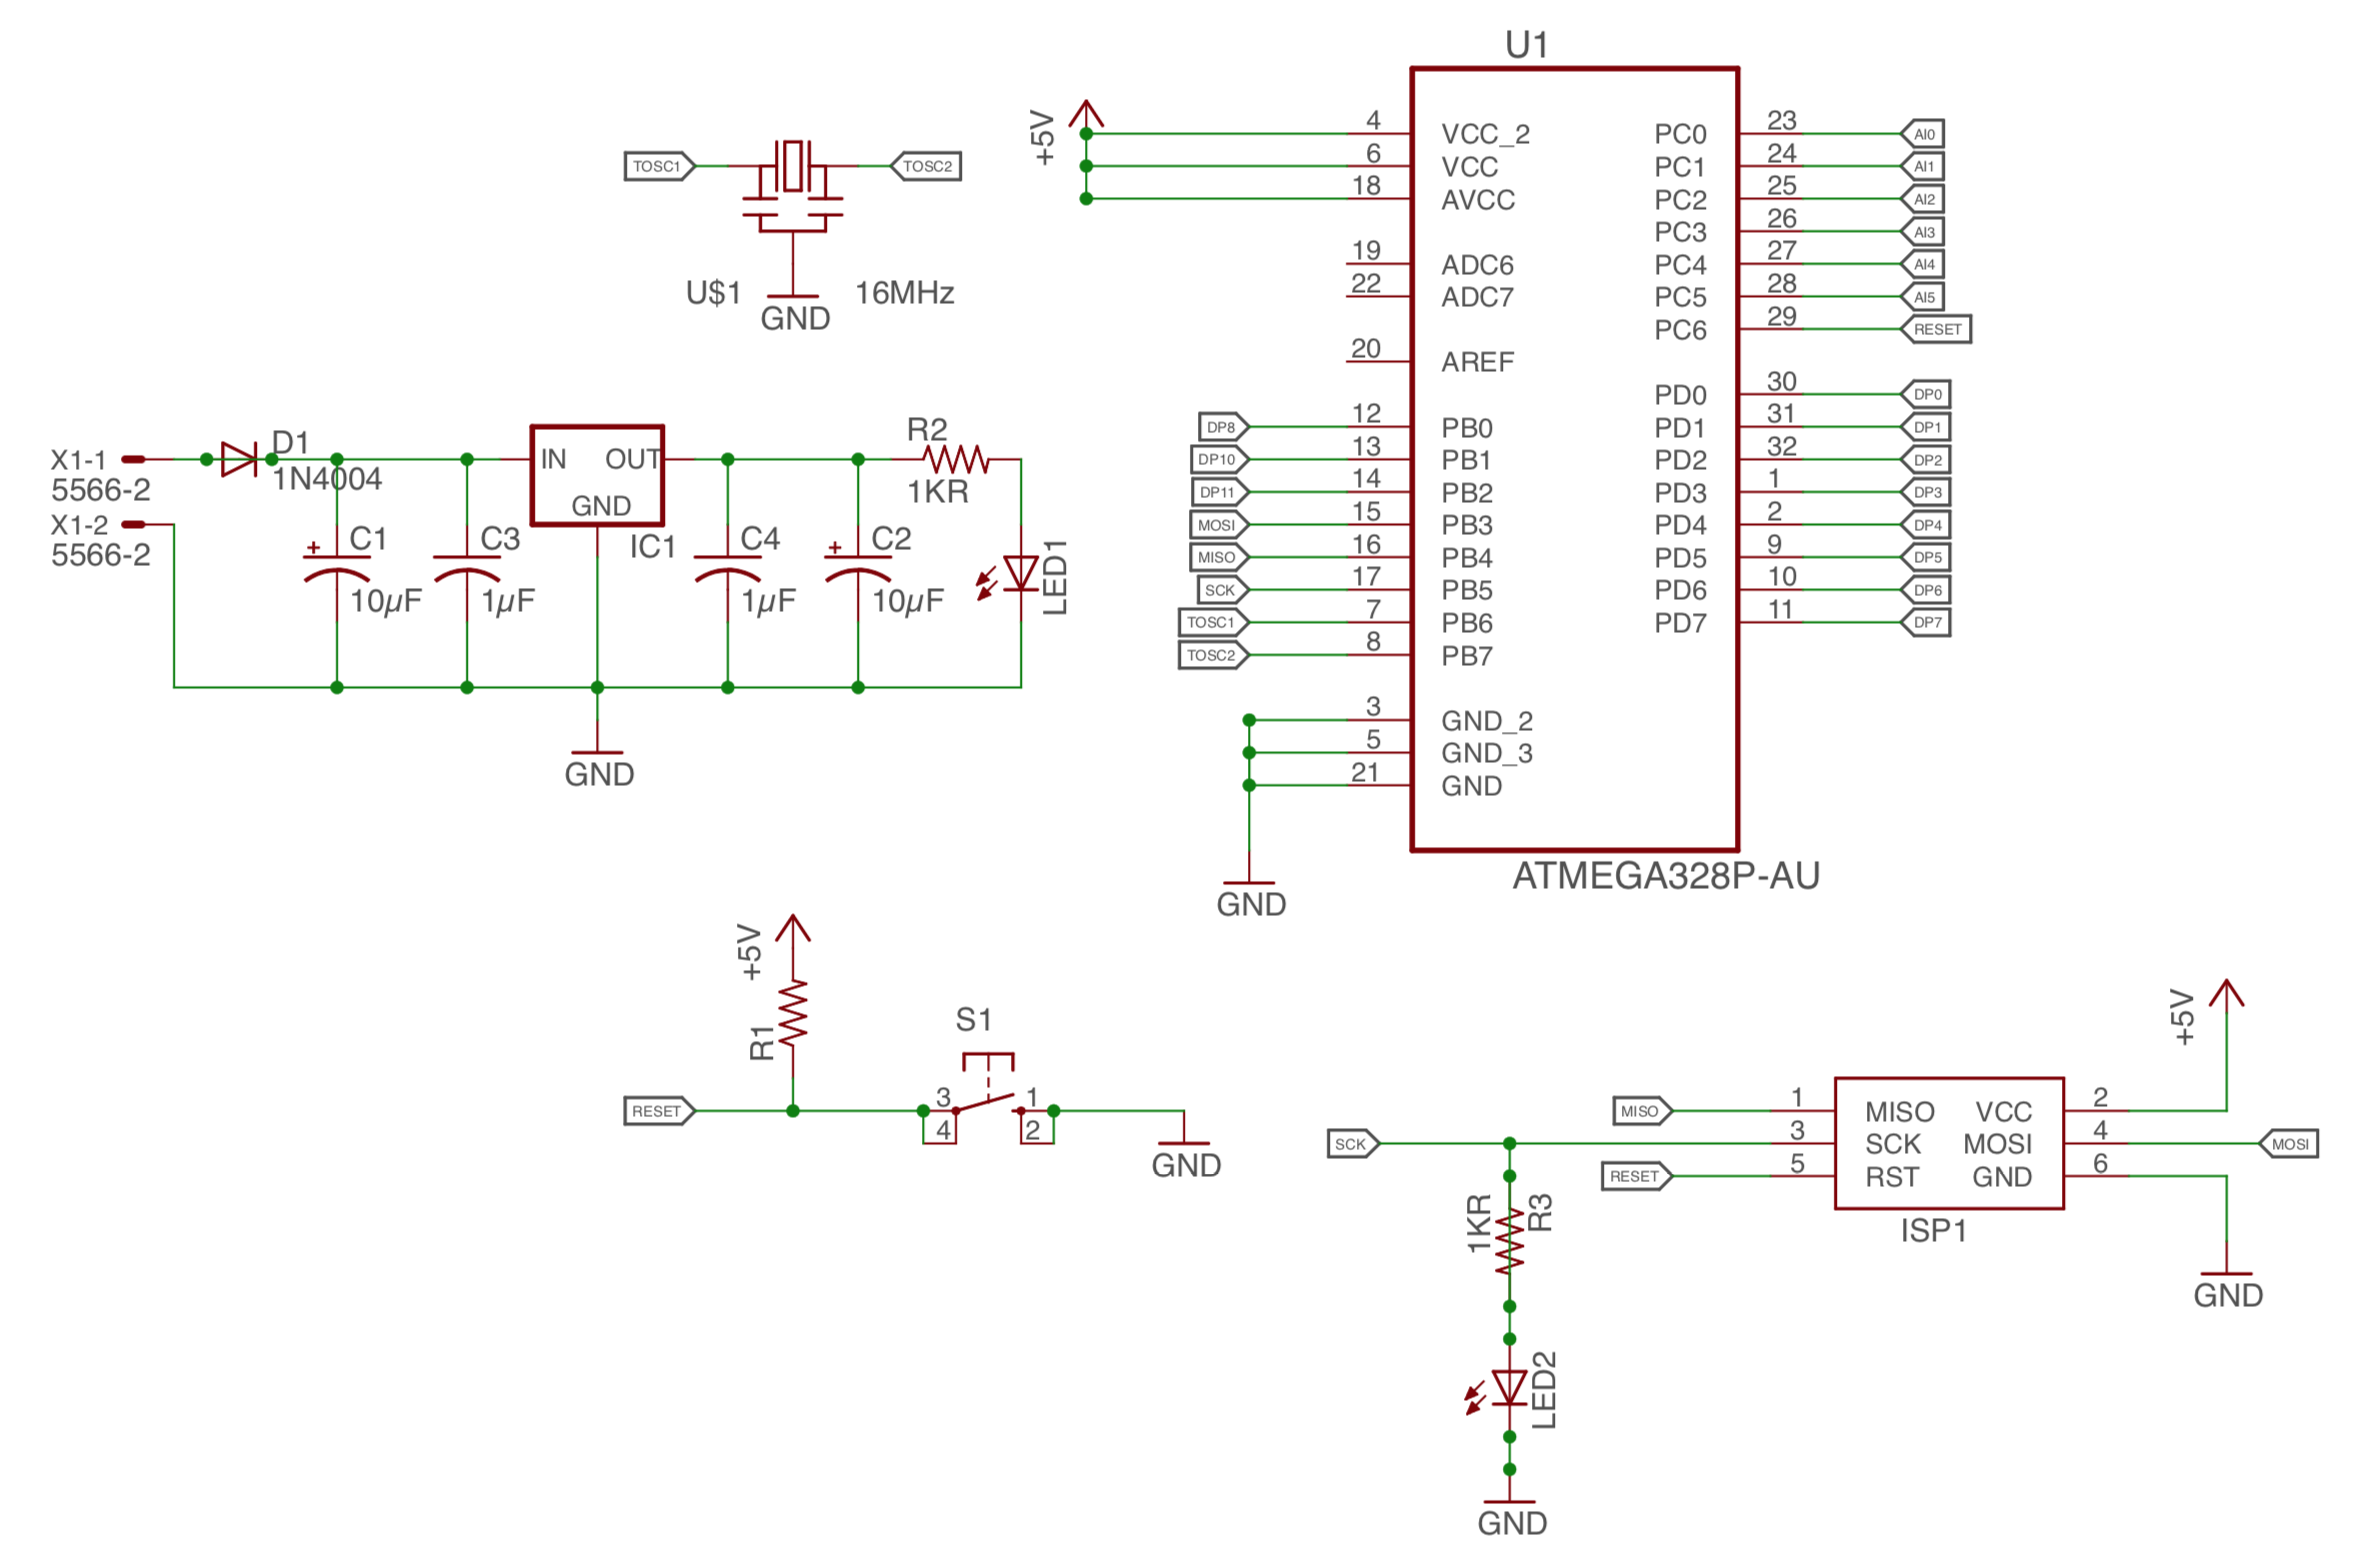
\includegraphics[scale=0.2]{atmega_schemat.png}
    \caption{Schemat}
    \label{fig:my_label}
\end{figure}
\end{frame}
\begin{frame}{Wyniki testowania}
    \begin{figure}[h]
    \centering
    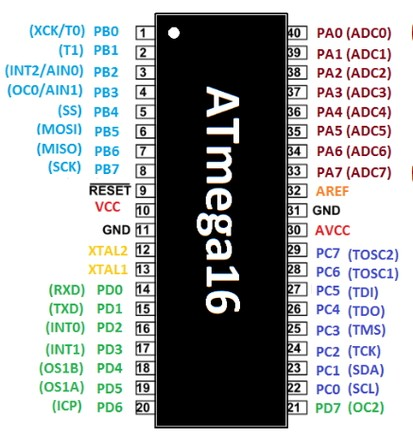
\includegraphics[scale=1]{atmega16.jpg}
    \caption{Atmega}
    \label{fig:my_label}
    \end{figure}
\end{frame}
\section{Podsumowanie}
\begin{frame}{Podsumowanie}
    Tutaj jakies podusowanie\\
    123
\end{frame}
\begin{frame}{Podsumowanie}
    \begin{math}
        x^{2y}\\
        log_2\\
        x^{y}_{1}\\[1cm]
        Wielokropki\\[1cm]
        \ldots
        \cdots
        \vdots
        \ddots\\[1cm] 
    \end{math}
\end{frame}
\begin{frame}{Podsumowanie}
    \begin{math}
            Inne\\
        \frac{(x+y)^2}{2x+b^2}\\[0.5cm]
        \sqrt[3]{20}\\[0.5cm]
        (a+b)^2 = a^2+2ab+b^2\\[0.5cm]
        \lim_{x\rightarrow 0}\\[0.5cm]
        \left\{\begin{array}{ccl}
             y&=&2x+3  \\
             y&=&3c-4
        \end{array}\right
    \end{math}
\end{frame}
\section{}
\begin{frame}{Podziękowanie}
    \begin{center}
        \textbf{{\large}Dziekuję za uwagę}
    \end{center}
\end{frame}
\end{document}
